%%%%%%%%%%%%%%%%%%%%%%%%%%%%%%%%%%%
%%  Einführung
%%%%%%%%%%%%%%%%%%%%%%%%%%%%%%%%%%%
\chapter{Einführung}

Im Fachmodul geht es darum, die heutige Situation, das Problem der Situation und die Lösung zu erarbeiten. In der heutigen Situation wird beschrieben, welche Komponenten das Projekt hat, in diesem Fall die der Wetterstation in Arbon. Bei der Problemanalyse wird aufgezeigt mit welchen Problemen die Wetterstation zu kämpfen hat. Im letzen Schritt, werden dann die Möglichkeiten zur Problemlösung aufgezeigt. Dies heisst aber nicht, dass die Probleme schon gelöst werden und in der Bachelorarbeit "nur" noch Programmiert bzw. eingebaut werden muss. Das Fachmodul wird folgende Komponenten enthalten:
 
\begin{itemize}  
\item Spezifikation
\item Risikoanalyse (Zeit, Umsetzung,..)
\item Entwicklungsprozess (z.B. V-Modell -> skizzieren)
\item Konzeptbeschreibung für die zu entwickelnden Artefakte
\item Konzept der Dokumenten- und Versionsverwaltung
\item Ein Dokument, welches die rechtlichen Ansprüche regelt
\item Ein Projektplan (Meilensteine)
\end{itemize}
\Diskussionspunkt{Ziel des Fachmoduls, Aufträge, Vorgehensweise, Vorstellung Wetterstation Arbon}

Die Wetterstation Arbon ist online erreichbar. Auf der Webseite der Station sind Informationen zum Wetter, Warnungen und die Geschichte der Station publiziert. Im Fachmodul, sowie später in der Bachelorarbeit wird nur ein Teil der Webseite und deren Komponenten gesprochen. Diese sind im Bild \ref{img:cms_struktur} auf Seite \pageref{img:cms_struktur} gelb umrandet. 
\begin{figure}[htbp]
	\centering
	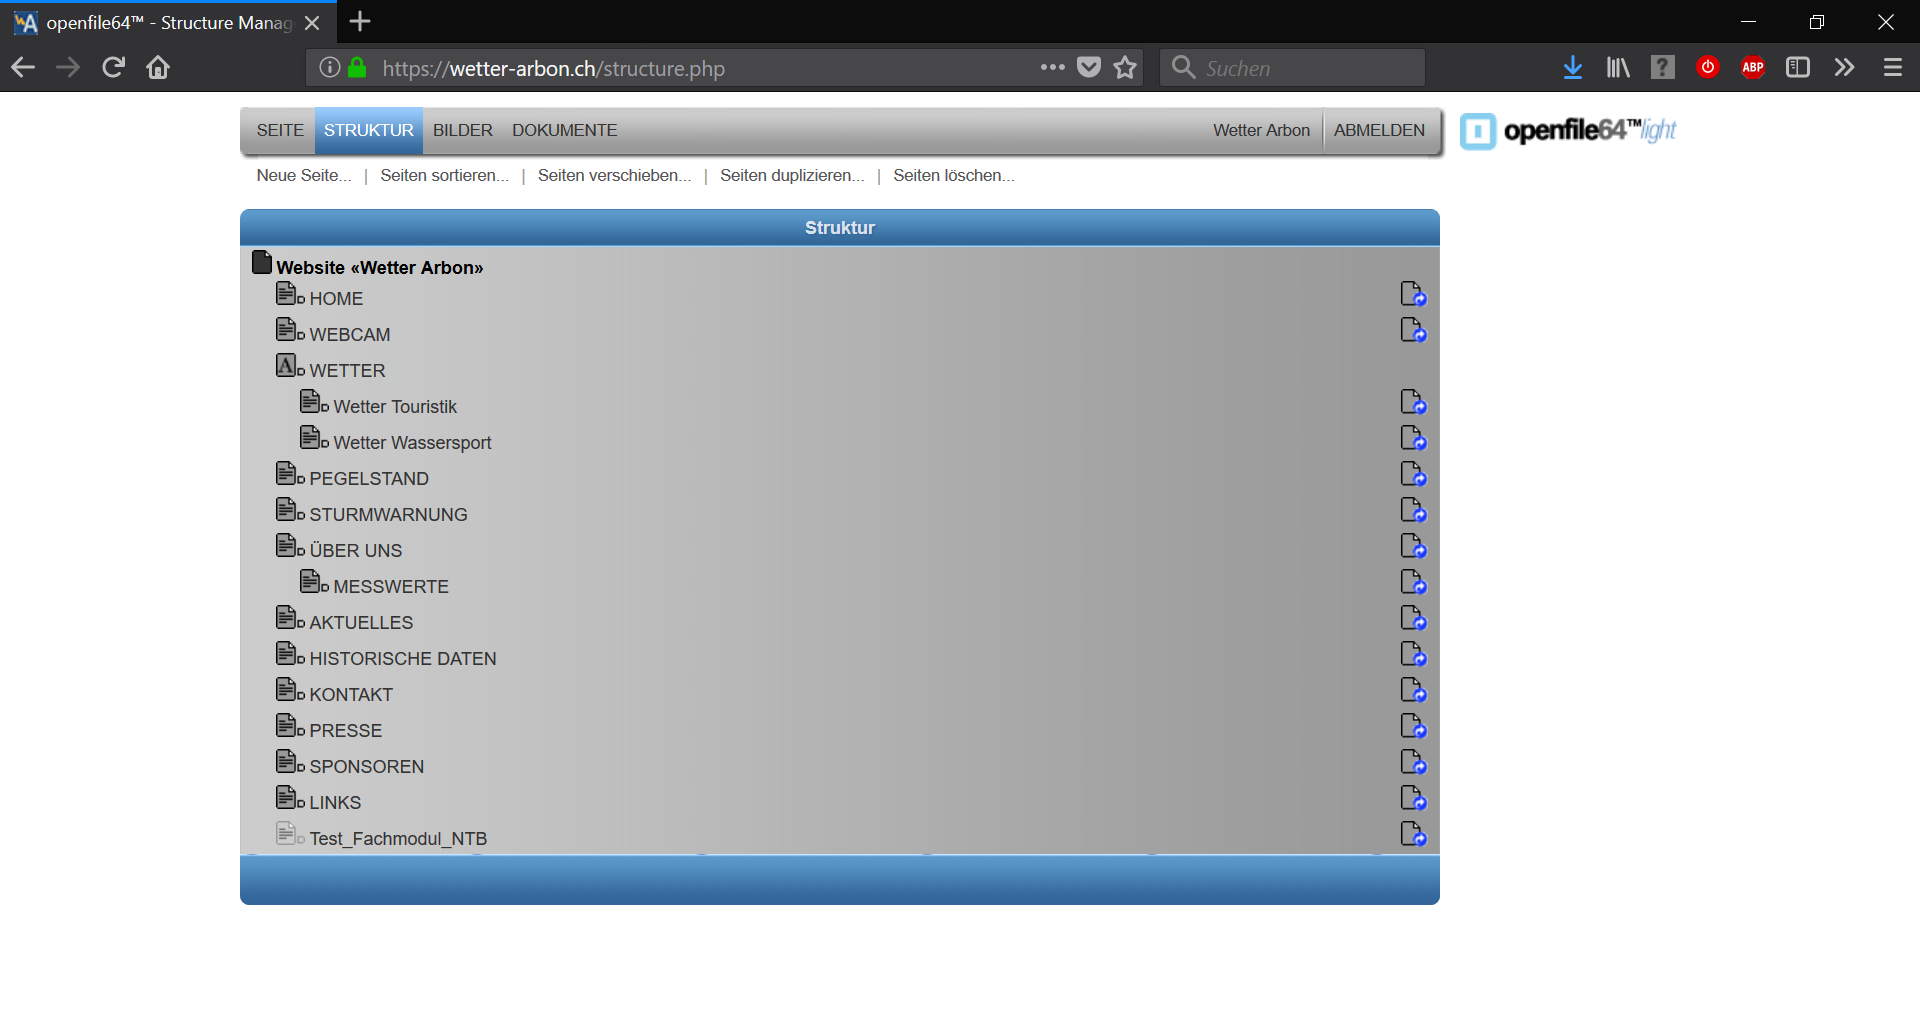
\includegraphics[width=0.9\linewidth]{img/cms_struktur}
	\caption{Struktur der Webseite sichtbar im CMS}
	\label{img:cms_struktur}
\end{figure}


\Diskussionspunkt{Foto Wetterstation}


\Diskussionspunkt{Beispiel für eine Bildintegration inkl. Referenz darauf:}
\begin{figure}[htbp]
	\centering
	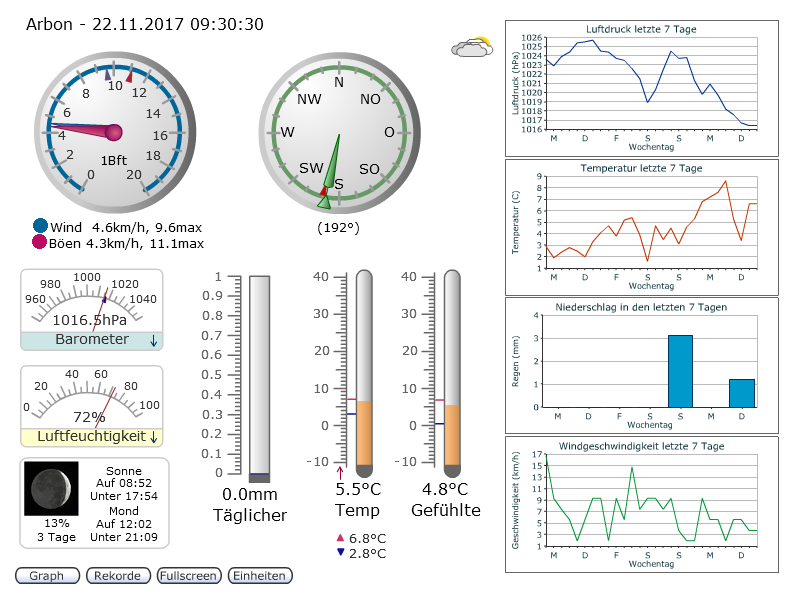
\includegraphics[width=0.9\linewidth]{img/grafik}
	\caption{eine Grafik ohne Sinn und Verstand}
	\label{img:grafik-dummy}
\end{figure}

Weiterhin wollen wir an dieser Stelle Bezug auf die Grafik
\ref{img:grafik-dummy} auf Seite \pageref{img:grafik-dummy} nehmen, was uns
hiermit gelungen sein dürfte. Latex passt die Seitenzahl aber auch die Nummer
der Grafik automatisch an, wir müssen uns um nichts kümmern.